\section{Pájecí pasty}
-základní složení, srovnání olovnatých a bezolovnatých slitin, tavidla

\subsection{Složení}
Pájecí pasta se skládá z mikroskopických kuliček pájky, které jsou pokryty vrstvou
kysličníku, tavidla, aktivátoru a technologické složky, která vytváří ze směsi pastu s
požadovanou viskozitou.
Pájecí pasta se skládá ze tří základních složek, kterými jsou:
\subsubsection{Pájecí materiály}
-cca 90 \%\\
Pro většinu povrchových montáží se dnes již používají bezolovnaté pasty.

\subsubsection{Tavidlo}
-cca 6 \%\\
Podle tavidla obsaženého v pastě rozdělujeme pasty na několik typů. Toto
rozdělení odpovídá kategoriím u tekutých pájecích tavidel, jež zahrnují kalafunu,
přírodní nebo syntetické pryskyřice a organické látky. Nejoblíbenější tavidla jsou
typu “no-clean“ nebo s nízkým zůstatkem nečistot -zbytků tavidla po tepelné reakci
(odpadá starost s čištěním). Používaná jsou i tavidla na základě organických
kyselin (OA).

\subsubsection{Pojivová složka}
-cca 4 \%\\
Pojivové složky jsou chemicky složitější, většinou tekutá, avšak nejsou schopna
zajistit (nastavit) viskozitu na požadovanou hodnotu. Kromě rozpouštědel a
aktivátorů jsou obsažena v pastě navíc materiály pro úpravu viskozity
(zahušťovadla) a teplotní stabilizátory. Zahušťovadla mají tu funkci, že pájecí
prášek zůstává přichycen na tavidle a neodděluje se od něj. Teplotní stabilizátory
zajišťují neměnnost vlastností pájecí pasty během přetavovacího procesu.

\begin{figure}[h]
   \begin{center}
     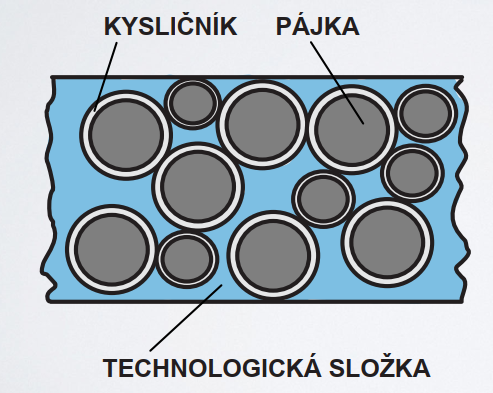
\includegraphics[scale=0.6]{images/Pasta.png}
   \end{center}
   \caption{Složení pájecí pasty}
\end{figure}
\pagebreak
\subsubsection{Oxidace}
 Forma a stupeň oxidace jsou důležité fyzikální vlastnosti pájecího prášku. Pro pájecí pastu
musí být použit pouze kulový prášek. Prášek, jehož odchylka od přesného tvaru koule je
větší než 4 \% je nevhodný. Použitím optického zobrazení je možno laboratorně měřit
několik vlastností pájecích past současně. Pomocí optického zobrazení vybraného počtu
částic lze určit velikost, tvar a rozložení – důležité vlastnosti ke správnému nanesení
pájecí pasty přes šablonu.

Stupeň oxidace popisuje nevodivá vrstva, která se vytvoří na povrchu pájecího prášku,
obsahuje uhličitany a sulfidy, které mohou ovlivnit viskozitu pasty, její schopnost tavení,
tvorbu kapek a také její životnost. Obvykle, pájecí prášek obsahuje 0,05 - 0,25 objemových
procent oxidantu

\subsection{Srovnání olovnatých a bezolovnatých slitin}
\textbf{Bezolovnaté}-vyšší teplota pájení, větší tendence k oxidaci, netoxické, přesnější nastavení pájecích parametrů, některé druhy křehké (Sn/Bi). (Sn100C - 217 $^{\circ}$C, Sn96,5/Ag3/Cu0,5 - 217 $^{\circ}$C)\\
\textbf{Olovnaté}-nižší teplota pájení, toxické, velmi dobré smáčecí charaktereistiky, nevytváří křehké intermetalické fáze. Sn63/Pb37 183 $^{\circ}$C.
\begin{figure}[h]
   \begin{center}
     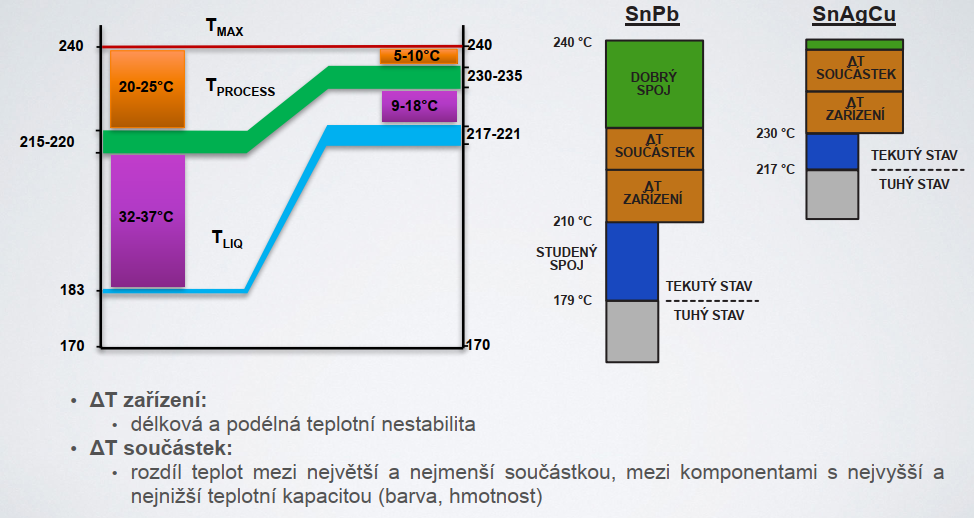
\includegraphics[scale=0.6]{images/Okno.png}
   \end{center}
   \caption{Procesní okno}
\end{figure}

\subsection{Tavidla}
\subsubsection{Funkce tavidla}
\begin{itemize}
\item odstraňuje povrchové oxidy a další nečistoty
\item odstraňuje a chrání před oxidací a brání přístupu reakčních prvků
\item napomáhá přestupu a rovnoměrnému rozložení tepla
\item vytváří prostředí s nízkým povrchovým napětím a zlepšuje smáčivost spojovaných
povrchů
\end{itemize}

Pokud je pájka dodávána jako pájecí pasta, je tavidlo smíšeno s částicemi pájky tak, že
pasta tvoří homogenní materiál. V případě pájek „trubičkových“ je tavidlo náplní trubičky.

Smáčením (v zásobníku s tekutým tavidlem je vytvořena vlna, která smáčí povrch spodní desky
plošného spoje. Za vlnou následuje měkký kartáč, který otírá přebytek tavidla z povrchu. Po nanesení
je tavidlo sušeno při teplotě 80-110 $^{\circ}$C)

Nanášením ve spreji (jedná se o klasický proces známý např. z nanášení barev tímto způsobem)

Nanášením pěny (využívá se probublávání plynu zásobníkem, ve kterém se nachází tavidlo. Na
povrchu tavidla se vytváří bublinky, které se nanášejí na povrch desky. Při praskání bublinek dochází
ke smáčení povrchu tavidlem a zároveň se podporuje čistící účinek tavidla)

\subsubsection{Typy tavidel}

\textbf{Tavidla rozpustná rozpouštědlem} (kalafuna + aktivátory, syntetická t.)\\
R, RMA, RA, RSA (fosfátové směsi)

Např. tavidlo RMA je tvořeno kalafunou rozpuštěnou v ředidle doplněnou aktivátorem,
kterým bývá organická kyselina nebo sůl. Poměr obsahu aktivátoru k obsahu ředidla
určuje aktivitu a tím i korozivitu tavidla. Typické pro tavidlo je, že maximální aktivitu vykazuje během pájecího procesu. Po zapájení spoje vykazuje tento typ tavidla velice
nízkou aktivitu a tím i korozivitu, a proto po zapájení spojů je nutné čištění.

\textbf{Tavidla rozpustná ve vodě} ( až 40 \% organické kyseliny)

\textbf{Tavidla bezoplachová} (1 – 5 \% organických kyselin, aminokyseliny)

Zákaz VOC - jsou těkavé organické sloučeniny, zjednodušeně řečeno organická rozpouštědla (složená z uhlíku, H3O a částečně z kyslíku, dusíku, síry, chlóru, brómu, fluoru).

Na bázi přírodní pryskyřice (RO)\\
Na bázi syntetické pryskyřice (RE)\\
Na bázi organické kyseliny (OR)\\

S mírou aktivace:\\
1) Nízká (LO ) - bez halogenidů\\
2) L1 - s 0,5 \% halogenidů\\
3) Střední M0, M1\\
4)Vysoká H0, H1\\









